\documentclass{beamer}
\usetheme{Copenhagen}
\usecolortheme{beaver}
\usepackage{pdfpages}
\usepackage[utf8]{inputenc}
\usepackage[portuges,brazil,english]{babel}
\usepackage{times}
\usepackage{epsfig}
\usepackage{graphicx}
\usepackage{amsmath}
\usepackage{amssymb}
\usepackage{color}
\usepackage{listings}
\usepackage[pagebackref=true,breaklinks=true,letterpaper=true,colorlinks,bookmarks=false]{hyperref}
%  ABACO -- Conjunto de macros para desenhar o 'abaco
%  Desenho original de Hans Liesenberg
%  Macros de Tomasz Kowaltowski
%  DCC -- IMECC -- UNICAMP
%  Mar,co de 1988  --  Vers~ao 1.0
% Ajustado para LaTeX da SUN -- Mar,co de 1991
% ---------------------------------------------------------
%  Chamada:   \ABACO{d1}{d2}{d3}{d4}{esc}
%             com:  di's -- os quatro d'igitos;
%                   esc  -- fator de escala
% ---------------------------------------------------------
%  DEFINI,C~OES AUXILIARES
% ---------------------------------------------------------
%  Forma o d'igito pequeno (0 ou 1)

\newcommand{\ABACODP}[1]{%
%
\thicklines
%    
\begin{picture}(8,0)
    \ifcase#1{   %  caso 0
       \put(0,0)    {\line(1,0){4}}
       \multiput(5,0)(2,0){2}{\oval(2,4)}}
    \or{         %  caso 1
       \put(2,0)    {\line(1,0){4}}
       \multiput(1,0)(6,0){2}{\oval(2,4)}}
    \fi
\end{picture}
    } % \ABACODP

% Forma o d'igito grande (0 a 4)

\newcommand{\ABACODG}[1]{%
%
\thicklines
%    
\begin{picture}(14,0)
    \ifcase#1{   % caso 0
       \multiput(1,0)(2,0){5}{\oval(2,4)}}
       \put(10,0)   {\line(1,0){4}}
    \or{         % caso 1
       \multiput(1,0)(2,0){4}{\oval(2,4)}}
       \put(8,0)   {\line(1,0){4}}
       \put(13,0)   {\oval(2,4)}
    \or{         % caso 2
       \multiput(1,0)(2,0){3}{\oval(2,4)}
       \put(6,0)   {\line(1,0){4}}
       \multiput(11,0)(2,0){2}{\oval(2,4)}}
    \or{         % caso 3
       \multiput(1,0)(2,0){2}{\oval(2,4)}
       \put(4,0)   {\line(1,0){4}}
       \multiput(9,0)(2,0){3}{\oval(2,4)}}
    \or{         % caso 4
       \put(1,0)  {\oval(2,4)}}
       \put(2,0)   {\line(1,0){4}}
       \multiput(7,0)(2,0){4}{\oval(2,4)}
    \fi
\end{picture}
    } % \ABACODG
       
% Forma um d'igito (0 a 9)

\newcommand{\ABACOD}[1]{%
%
    \ifnum#1>9
       \errmessage{#1: Argumento invalido para ABACO}
    \fi
    \ifnum#1<0
       \errmessage{#1: Argumento invalido para ABACO}
    \fi
%
\begin{picture}(24,0)
%    
    \ifnum#1<5
       \put(16,0) {\ABACODP{0}}
    \else   
       \put(16,0) {\ABACODP{1}}
    \fi
%    
    \ifnum#1<5
       \put(0,0)  {\ABACODG{#1}}
    \else
       \ifcase#1\or \or \or \or
          \or  \put(0,0)  {\ABACODG{0}}
          \or  \put(0,0)  {\ABACODG{1}}
          \or  \put(0,0)  {\ABACODG{2}}
          \or  \put(0,0)  {\ABACODG{3}}
          \or  \put(0,0)  {\ABACODG{4}}
       \fi
    \fi   
\end{picture}
    } % \ABACOD
    
% -------------------------------------------------

%  DEFINI,C~AO PRINCIPAL
    
\newcommand{\ABACO}[5]{%
    \setlength{\unitlength}{#5mm}
%
    \thinlines
%   
\begin{picture}(28,25)
%   
% moldura
%
% externa
%
        \put(0,0)            {\line(0,1){25}}
        \put(0,0)            {\line(1,0){28}}
        \put(28,0)           {\line(0,1){25}}
        \put(0,25)           {\line(1,0){28}}
% interna
        \put(2,2)            {\line(0,1){21}}
        \put(26,2)           {\line(0,1){21}}
        \put(16,2)           {\line(0,1){21}}
        \put(18,2)           {\line(0,1){21}}
        \put(2,2)            {\line(1,0){14}}
%        \put(16,2)           {\line(1,-1){1}}
%        \put(17,1)           {\line(1,1){1}}
        \put(18,2)           {\line(1,0){8}}
        \put(2,23)           {\line(1,0){14}}
%        \put(16,23)          {\line(1,1){1}}
%       \put(17,24)          {\line(1,-1){1}}
        \put(18,23)          {\line(1,0){8}}
%        \put(0,0)            {\line(1,1){2}}
%        \put(0,25)           {\line(1,-1){2}}
%        \put(28,0)           {\line(-1,1){2}}
%        \put(28,25)          {\line(-1,-1){2}}
%
%   
% d'igitos
%
%   
       \put(2,20)  {\ABACOD{#1}}
       \put(2,15)  {\ABACOD{#2}}
       \put(2,10)  {\ABACOD{#3}}
       \put(2,5)   {\ABACOD{#4}}
%      
\end{picture}
    } % \ABACO
    

\usepackage[usenames,dvipsnames]{color}    
\usepackage[usenames,dvipsnames]{color}    
 \lstset{ 
  language=R,                     % the language of the code
  basicstyle=\footnotesize\ttfamily, % the size of the fonts that are used for the code
  numbers=left,                   % where to put the line-numbers
  numberstyle=\footnotesize\color{Blue},  % the style that is used for the line-numbers
  stepnumber=1,                   % the step between two line-numbers. If it's 1, each line
                                  % will be numbered
  numbersep=5pt,                  % how far the line-numbers are from the code
  backgroundcolor=\color{white},  % choose the background color. You must add \usepackage{color}
  showspaces=false,               % show spaces adding particular underscores
  showstringspaces=false,         % underline spaces within strings
  showtabs=false,                 % show tabs within strings adding particular underscores
  frame=single,                   % adds a frame around the code
  rulecolor=\color{black},        % if not set, the frame-color may be changed on line-breaks within not-black text (e.g. commens (green here))
  tabsize=2,                      % sets default tabsize to 2 spaces
  captionpos=b,                   % sets the caption-position to bottom
  breaklines=true,                % sets automatic line breaking
  breakatwhitespace=false,        % sets if automatic breaks should only happen at whitespace
  keywordstyle=\color{RoyalBlue},      % keyword style
  commentstyle=\color{YellowGreen},   % comment style
  stringstyle=\color{ForestGreen}      % string literal style
} 
\cvprfinalcopy % *** Uncomment this line for the final submission
\def\httilde{\mbox{\tt\raisebox{-.5ex}{\symbol{126}}}}
\ifcvprfinal\pagestyle{empty}\fi

\newcommand{\TODO}[1]{TODO: #1}
\newcommand{\CITEONE}[2]{\mbox{#1 \cite{#2}}}
\newcommand{\CITETWO}[3]{\mbox{#1 and #2 \cite{#3}}}
\newcommand{\CITEN}[2]{\mbox{#1 et al. \cite{#2}}}

%\setbeamercolor{alerted text}{fg=orange}
%\setbeamercolor{background canvas}{bg=white}
%\setbeamercolor{block body alerted}{bg=normal text.bg!90!black}
%\setbeamercolor{block body}{bg=normal text.bg!90!black}
%\setbeamercolor{block body example}{bg=normal text.bg!90!black}
%\setbeamercolor{block title alerted}{use={normal text,alerted text},fg=alerted text.fg!75!normal text.fg,bg=normal text.bg!75!black}
%\setbeamercolor{block title}{bg=blue}
%\setbeamercolor{block title example}{use={normal text,example text},fg=example text.fg!75!normal text.fg,bg=normal text.bg!75!black}
%\setbeamercolor{fine separation line}{}
%\setbeamercolor{frametitle}{fg=brown}
%\setbeamercolor{item projected}{fg=black}
%\setbeamercolor{normal text}{bg=black,fg=blue}
%\setbeamercolor{palette sidebar primary}{use=normal text,fg=normal text.fg}
%\setbeamercolor{palette sidebar quaternary}{use=structure,fg=structure.fg}
%\setbeamercolor{palette sidebar secondary}{use=structure,fg=structure.fg}
%\setbeamercolor{palette sidebar tertiary}{use=normal text,fg=normal text.fg}
%\setbeamercolor{section in sidebar}{fg=brown}
%\setbeamercolor{section in sidebar shaded}{fg=grey}
%\setbeamercolor{separation line}{}
%\setbeamercolor{sidebar}{bg=red}
%\setbeamercolor{sidebar}{parent=palette primary}
%\setbeamercolor{structure}{bg=black, fg=green}
%\setbeamercolor{subsection in sidebar}{fg=brown}
%\setbeamercolor{subsection in sidebar shaded}{fg=grey}
%\setbeamercolor{title}{fg=brown}
%\setbeamercolor{titlelike}{fg=brown}

\title[Child stuntedness] % (optional, only for long titles)
{Child stuntedness}
\subtitle{An overview from Machine Learning}
\author[Author, Anders] % (optional, for multiple authors)
{F.~Brolesi\inst{1} \and F.~Luz\inst{2}}
\institute[Universities Here and There] % (optional)
{
  \inst{1}%
  Is with the Institute of Computing \\
  University of Campinas (Unicamp\footnote{\url{http://www.unicamp.br/unicamp/}})
  \and
  \inst{2}%
  Is with the Institute of Computing\\
  University of Campinas (Unicamp)
}
\date[KPT 2004] % (optional)
{State University of Campinas, 2014}
\subject{Computer Science}
\begin{document}
\frame{\titlepage}

\begin{document}
  \begin{frame}
    \frametitle{Growth stunting}
    ``Growth stunting is defined by comparing measurements of children's heights to the NCHS\footnote{National Center for Health Statistics} growth reference population: children who fall below the fifth percentile of the reference population in height for age are defined as stunted. As an indicator of nutritional status, comparison of children's measurements with growth reference curves may be used differently for populations of children than for individual children. However, if substantially more than 5\% of an identified child population have height for age that is less than the fifth percentile on the reference curve, then the population is said to have a higher-than-expected prevalence of stunting, and inadequate nutrition is generally the first cause considered."
  \end{frame}
  \begin{frame}
    \frametitle{Child malnutrition}
    \framesubtitle{Stunting trending}
			\begin{figure}
			\begin{center}
				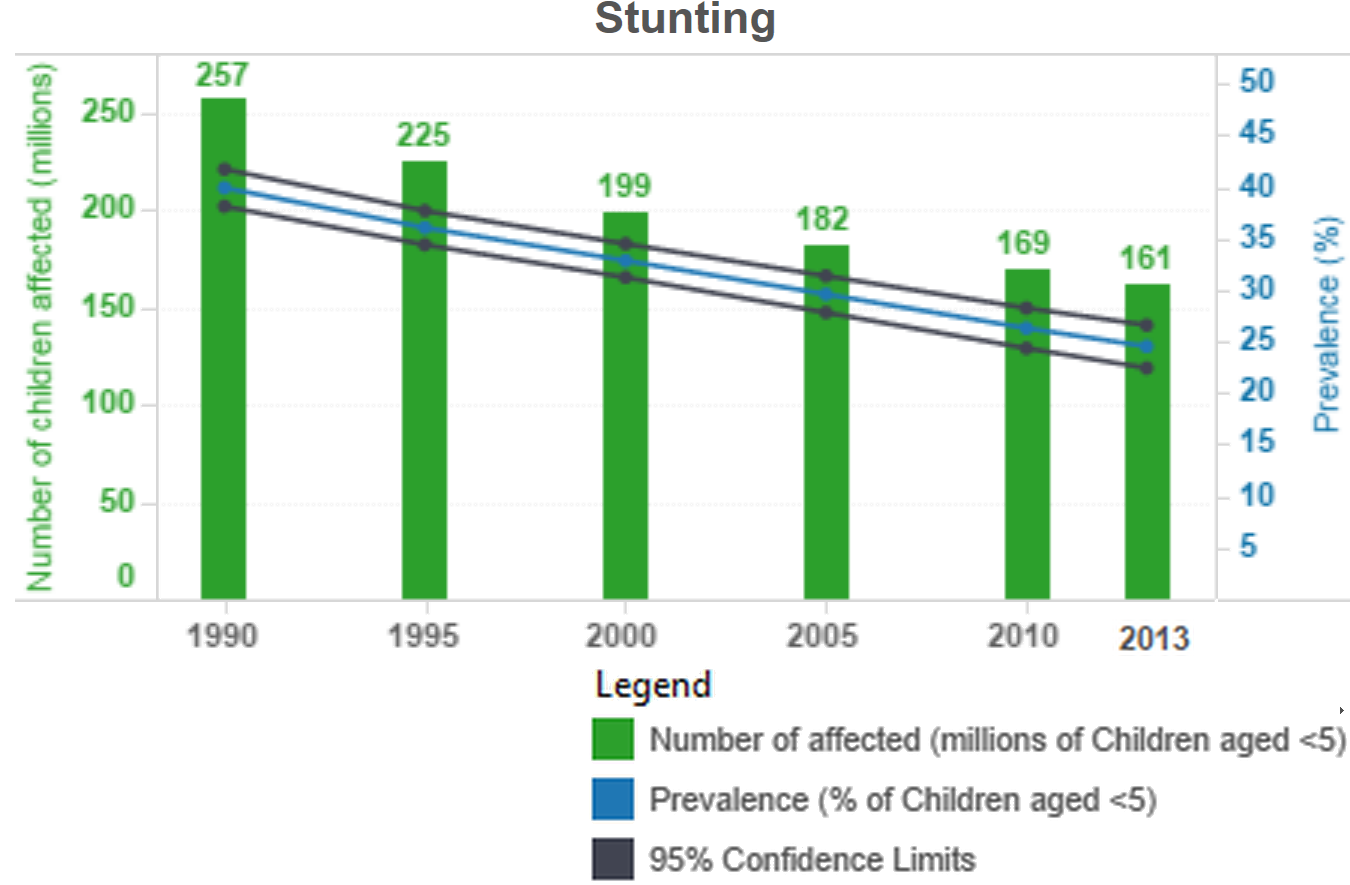
\includegraphics[width=0.99\columnwidth]{pics/unicef01}
				\caption{\small{Child malnutriotion trend for stunting (According to Unicef).}}  
			\end{center} 
			\end{figure}  
  \end{frame}
\begin{frame}
\frametitle{Stunting around the world}
 \begin{figure}
\begin{center}
	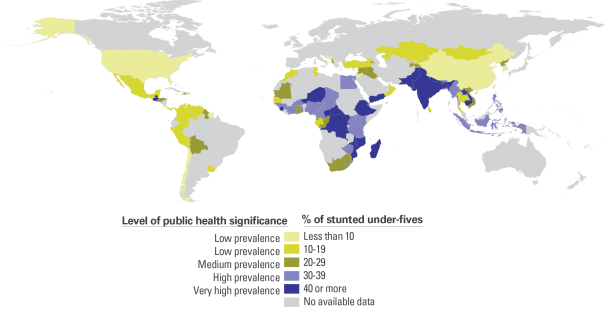
\includegraphics[width=0.99\textwidth]{pics/unicef02}
	\caption{\small{Undernutrition contributes to half of all deaths in children under 5 and is widespread in Asia and Africa
Percentage of under-five children who are stunted, 2008 - 2013).}}   
\end{center} 
\end{figure}  
\end{frame}	

\begin{frame}
\frametitle{Problem statement}
Using the statement described in \cite{topcoder}, we have the goal to determine a combination of early measures that would be a good predictor for birth weight. In pursuit of this goal, we have collected time series data from ultrasounds on pregnant mothers. We would like you to use this data to predict a child’s birth weight and birth date (days from pregnancy start).

For each fetus given sex, status, and multiple ultrasound measurements(columns 5-12) during the pregnancy (time being the variable t.ultsnd). The data from the repeated ultrasounds provides a small time series that can be used for predicting the birth weight and day.

\end{frame}

\begin{frame}
\frametitle{Dataset}
\begin{figure}
\begin{center}
	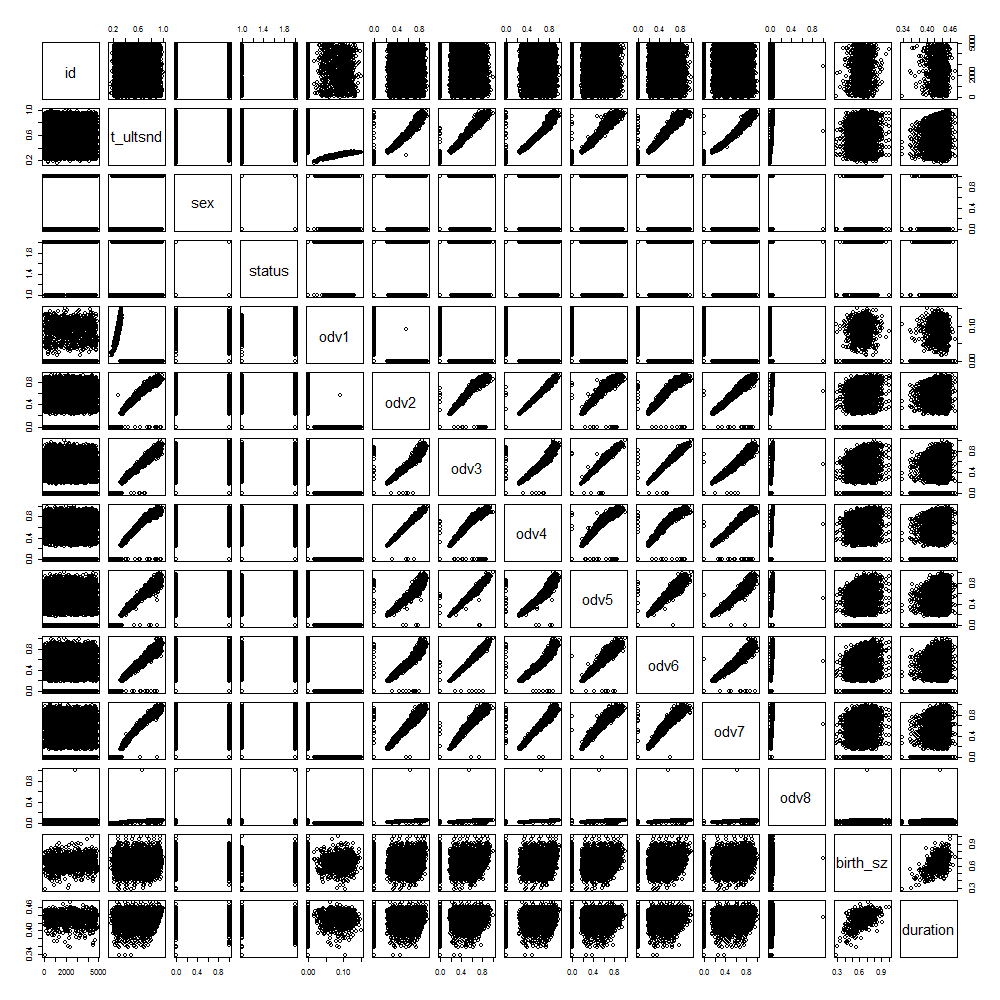
\includegraphics[width=0.75\textheight]{pics/plot-data-1000}
	\caption{The whole dataset plotted.\label{fig:dataset_full}}   
\end{center} 
\end{figure}  
\end{frame}

\begin{frame}
\frametitle{Dataset}
\begin{figure}
\begin{center}
	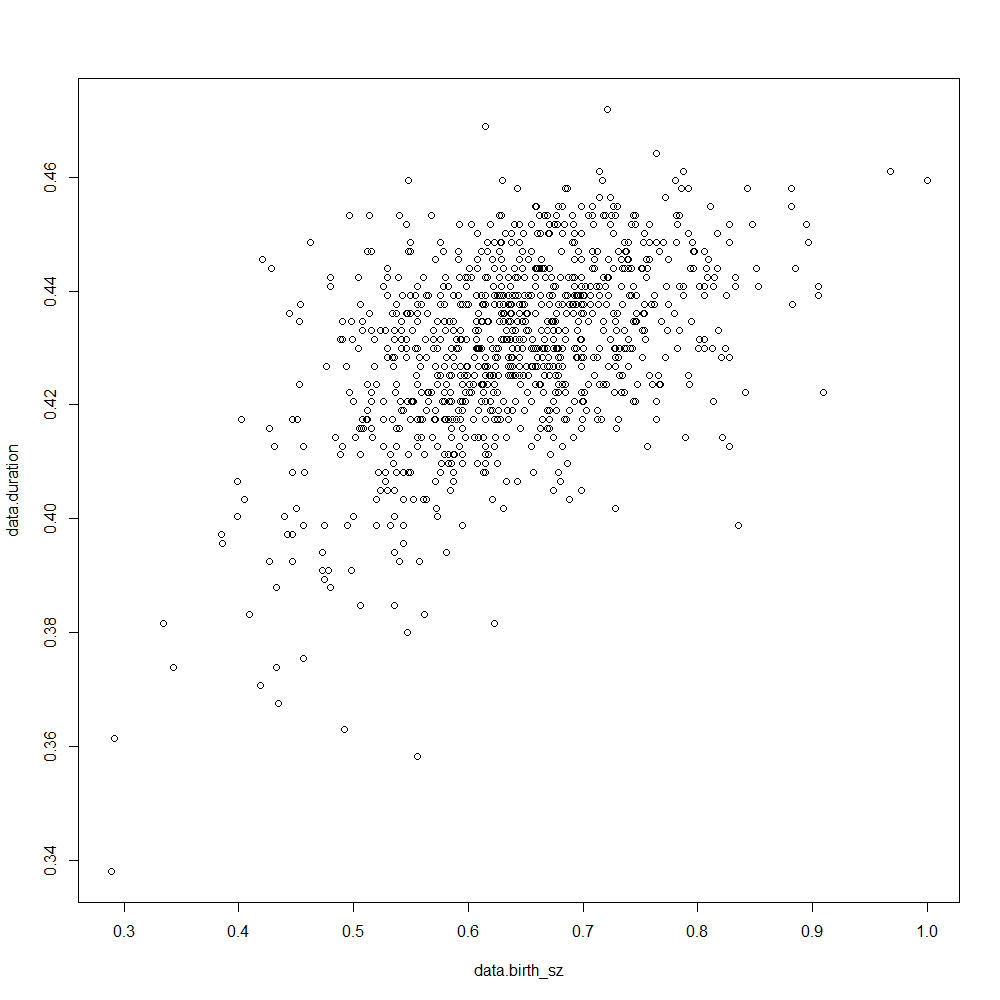
\includegraphics[width=0.66\columnwidth]{pics/birth_vs_duration}
	\caption{Birth vs Duration plot according the dataset.\label{fig:birth_vs_duration}}   
\end{center} 
\end{figure}  
\end{frame}	

\begin{frame}
\frametitle{Further studies}
There's a lot of ways to understand the problem of stunting in child populations. The website Topcoder\footnote{\url{https://www.topcoder.com/}} recently released another two problems regarding this issue \footnote{\url{http://community.topcoder.com/longcontest/?module=ViewProblemStatement&rd=16153&pm=13478} and \url{https://www.topcoder.com/longcontest/?module=ViewProblemStatement&rd=16209&compid=45332}}.

Some ways of understand of how to deal this problem permeates the ethnic differences, for instance.
\end{frame} 
\begin{frame}
\frametitle{Further studies}
This work clearly does not contain all the possibilities and variations that may occur in relation to the subject of malnutrition and stunting. The possibilities of dealing with this subject are diverse, so we propose the extrapolation to this discipline and continue the development of intelligent algorithms that can be in support of medical decisions to inform pregnant women about the nutrition of their children.
\end{frame}

\begin{frame}
\nocite{*}
\frametitle{References}
{\small
\bibliography{refs}
}
\end{frame}	

	
% etc
\end{document}
\end{document}